\documentclass[../../main]{subfiles}

\renewcommand\thesection{\arabic{section}}


\begin{document}

\section{ESP32} \label{sec:}

\begin{center}
    {\begin{minipage} [c] {0.55\textwidth}
        \esp is a well \emph{documented} and a \emph{powerful} \emph{micro-controller} available in
        the market. The \emph{Espressif}\footnote{see footnote \ref{fnt:espressif}.} makes a wide verity
        of micro-controllers, the one we have chosen is the \esp. And \esp comes in different \emph{dev
        boards}. From those we will be using the board \texttt{ESP32-D0WD-V3}.

        Please refer figure \ref{fig:esp32DevBoard} and \ref{fig:esp32PinDiagram} for a quick glance
        at the device. And table \ref{tbl:esp32ReleventPins} gives a brief information about some
        relevant pins.
    \end{minipage}
    \hfill
    \begin{minipage} [c] {0.35\textwidth}
        \centering
        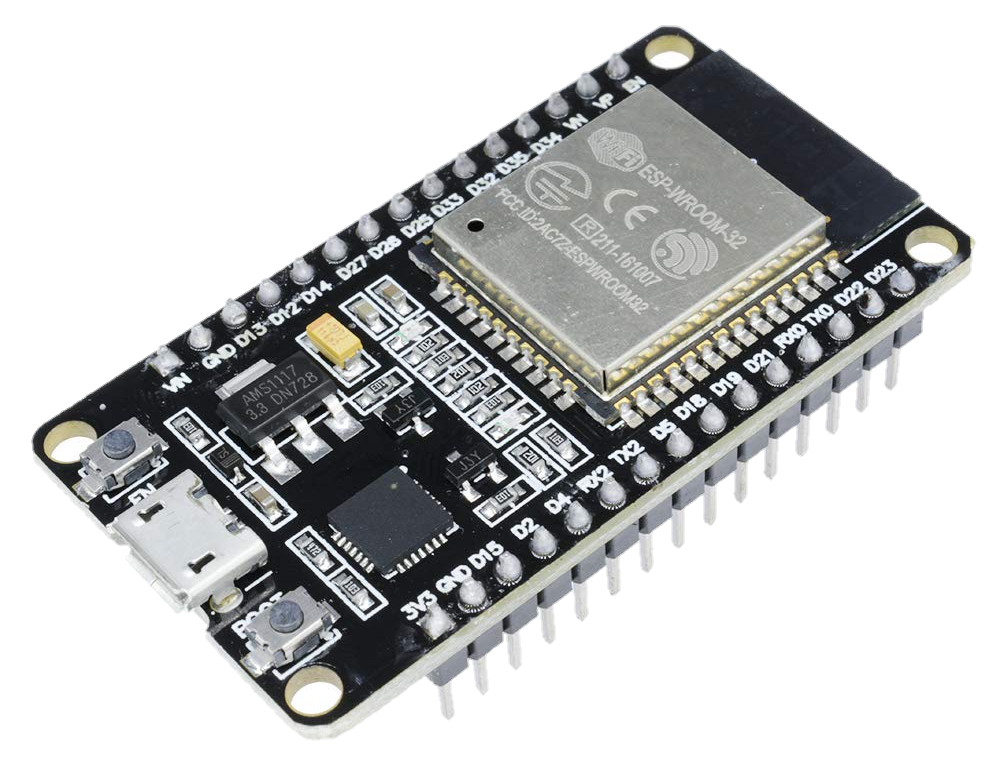
\includegraphics [
            max width = \IGXMaxWidth,
            max height = \IGXMaxHeight,
            \IGXDefaultOptionalArgs,
        ] {pics/esp32.png}
        \captionof{figure} {
            \esp \texttt{ESP32-D0WD-V3} board.
            \label{fig:esp32DevBoard}
        }
    \end{minipage}\hfill}
\end{center}


\begin{center}
    {\begin{minipage}[c] {0.42\textwidth}
        \centering

        \includegraphics [
            max width = \IGXMaxWidth,
            max height = \IGXMaxHeight,
            \IGXDefaultOptionalArgs,
        ] {tikzpics/endAbsESPPinout.pdf}
        \captionof{figure} {
            Pin diagram of \texttt{ESP32-D0WD-V3} Board.
            \label{fig:esp32PinDiagram}
        }

    \end{minipage}
    \begin{minipage}[c] {0.52\textwidth}

        \begin{center}
            \begin{tabularx} {\linewidth} {
                    *{1}{>{\centering\arraybackslash}m{0.5\linewidth}}
                    *{1}{>{\centering\arraybackslash}m{0.5\linewidth}}
                }
                \toprule
                Pins & Remarks \\
                \midrule
                \texttt{C0 - C15} & $16$ channel lines. \\
                \texttt{S0 - S3} & $4$ select lines. \\
                $\overline{\mbox{\texttt{E}}}$ & Enable line. \\
                \texttt{SIG} & Signal line. \\
                \bottomrule
            \end{tabularx}
            \captionof{table} {
                Relevant pins of \esp.
                \label{tbl:esp32RelventPins}
            }
        \end{center}

    \end{minipage}}

\end{center}

\end{document}
